\documentclass[conference]{IEEEtran}
\usepackage{cite}
\usepackage{amsmath,amssymb,amsfonts}
\usepackage{algorithmic}
\usepackage{graphicx}
\usepackage{textcomp}
\usepackage{xcolor}
\def\BibTeX{{\rm B\kern-.05em{\sc i\kern-.025em b}\kern-.08em
    T\kern-.1667em\lower.7ex\hbox{E}\kern-.125emX}}
\begin{document}

\title{100W Low Voltage AC-DC Converter\\}


\author{\IEEEauthorblockN{Chasen Gaither}
\IEEEauthorblockA{\textit{Student ID: 1974745} \\
\textit{University of Washington}\\
Seattle, WA, USA \\
chasennn@uw.edu}
\and
\IEEEauthorblockN{Khushbu Patel}
\IEEEauthorblockA{\textit{Student ID: 2400367} \\
\textit{University of Washington}\\
Seattle, WA, USA \\
kbupatel@uw.edu}
\and
\IEEEauthorblockN{Enrique Antunano}
\IEEEauthorblockA{\textit{Student ID: 2400331} \\
\textit{University of Washington}\\
Seattle, WA, USA \\
enriantu@uw.edu}
}

\maketitle

\begin{abstract}
This document covers the design of a DO-160G EMI Category L, M, H compliant AC-DC converter that accepts a 115 \textit{Vac}, 400 \textit{Hz}, voltage input
and can provide up to 100 \textit{W} to a 28 \textit{Vdc} output.
\end{abstract}

\section{Introduction}
This document covers the design of a DO-160G EMI compliant AC-DC converter that accepts a 115 \textit{Vac}, 400 \textit{Hz}, voltage input
and can provide up to 100 \textit{W} to a 28 \textit{Vdc} output. The power path will require AC rectification and a DC step-down with a buck converter. As the team's experience is in the aerospace industry, DO-160G EMI requirements will be used instead of FCC or CISPR requirements. DO-160G covers the compliance of aircraft equipment with multiple environmental and electromagnetic conditions found in aircraft. DO-160G is referenced by the FAA’s Advisory Circular AC 21-16G and other regulatory authorities worldwide. Our group decided to pursue an aerospace standard since all three members on the team work in the aerospace industry and find the experience valuable for their own professional growth.

\section{EMI Compliance Standard}

The design standard our team will adhere to is the DO-160G standard for Category L, M, and H electronics. DO-160G is maintained by the Radio Technical Commission for Aeronautics (RTCA). Category L, M, and H cover electronics that are far from apertures of an aircraft, near apertures, and direct view of RF antennas of an aircraft. The DO-160G categories were selected because our team thought, given our knowledge and the time constraints of this course, we could design an AC-DC converter with a stricter EMI emissions limit without going to the extreme of the standard. As reference, category B is the least strict, categories L,M, and H are in the middle, and categories P and Q are the most strict. Additionally, our team will only be modeling the power rail behavior, thus we will ignore the EMI limits specified for Interconnecting Bundles.

\subsection{Conducted Emissions Requirement}

Conducted Emissions requirements are specified in RTCA / DO-160 Conducted Emissions testing, Section 21.0. The test's range of interest goes from 150${kHz}$ to 152${MHz}$.

See Figure \ref{fig:do-160g_conducted_emissions_limit_diagram} for a graph of the conducted emission limit for categories L, M, and H for power lines.

\begin{figure}[htbp]
    \centering
    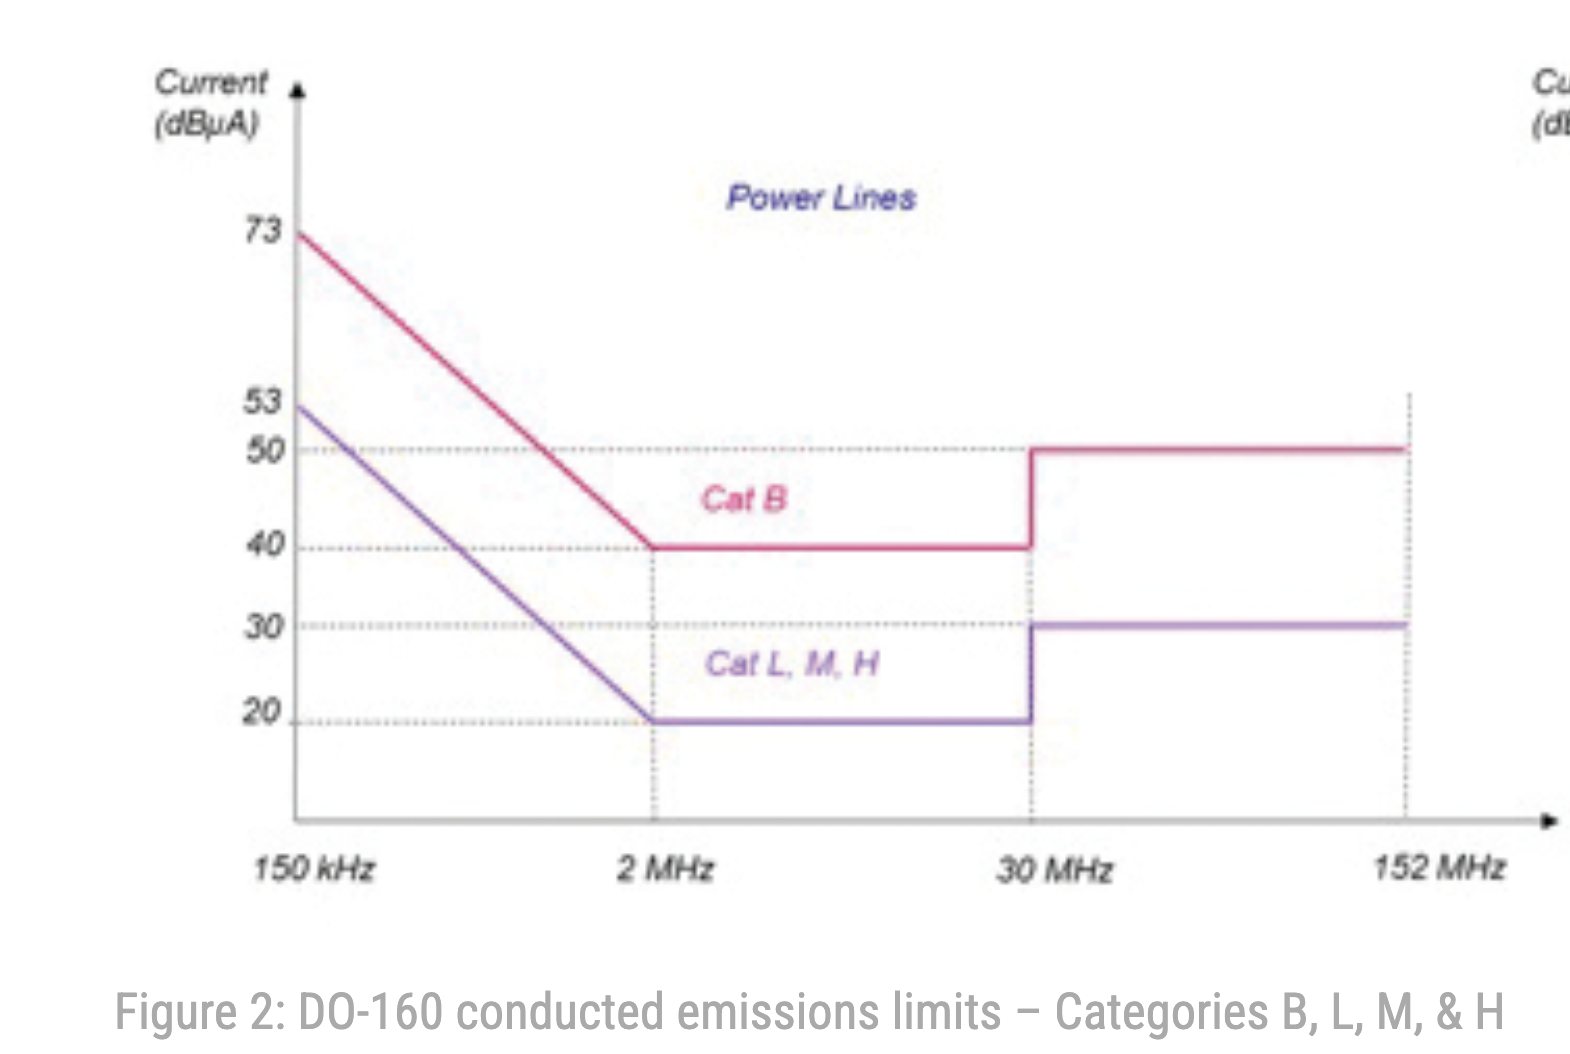
\includegraphics[width=1.0\linewidth]{do-160g_conducted_emissions_limit.png}
    \caption{DO-160G Conducted Emissions Limit for Category L, M, and H for Power Lines}
    \label{fig:do-160g_conducted_emissions_limit_diagram}
\end{figure}

\subsection{Direct Lightning Pin Injection Requirement}
Lightning induced transient susceptibility requirements are specified in RTCA / DO-160 Direct Lightning Pin Injection testing, Section 22.0. Indirect lightning testing will not be conducted, as these test requirements are for transient injection at the cable bundle, and the focus of this project is on the power rail of the equipment-under-test (EUT). Compliance will be conducted through LTSpice simulation of test injection waveforms specified by DO-160G, which provide a representation of a lightning strike. Direct pin injection testing for this project will be done with waveform set A, see Figure \ref{fig:do-160f_pin_injection_test_table} for the waveforms called out by set A. Set A will be used because set B specifies injection at a cable bundle rather than at the EUT pin. 

\begin{figure}[hp]
    \centering
    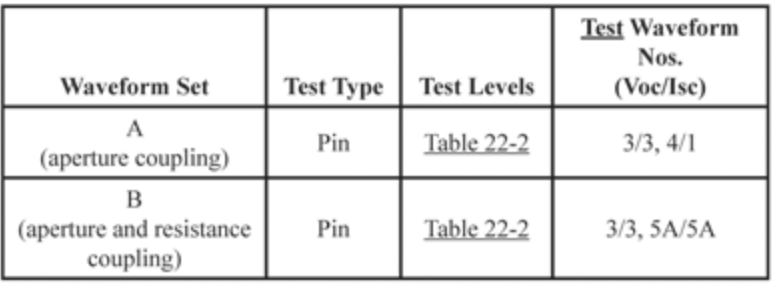
\includegraphics[width=1.0\linewidth]{do-160f_pin_injection_test_table.png}
    \caption{DO-160F Direct Pin Injection Lightning Test Table}
    \label{fig:do-160f_pin_injection_test_table}
\end{figure}

Set A's waveform 3 injects a damped oscillatory voltage and current waveform. See Figure \ref{fig:do-160f_waveform_set_3_diagram} for the waveform.

\begin{figure}[hp]
    \centering
    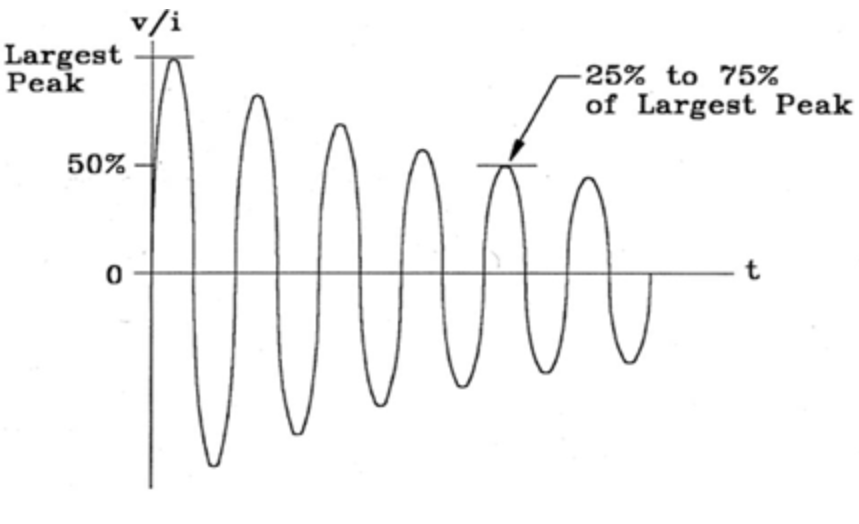
\includegraphics[width=1.0\linewidth]{do-160f_waveform_set_3.png}
    \caption{DO-160F Direct Pin Injection Lightning Test Waveform 3}
    \label{fig:do-160f_waveform_set_3_diagram}
\end{figure}

Set A's waveform 4 injects a peak voltage that peaks according to a time variable ${T1}$ and decays to 50\% of $V_{peak}$ by time ${T2}$. See Figure \ref{fig:do-160f_waveform_set_4_diagram} for the waveform.

\begin{figure}[hp]
    \centering
    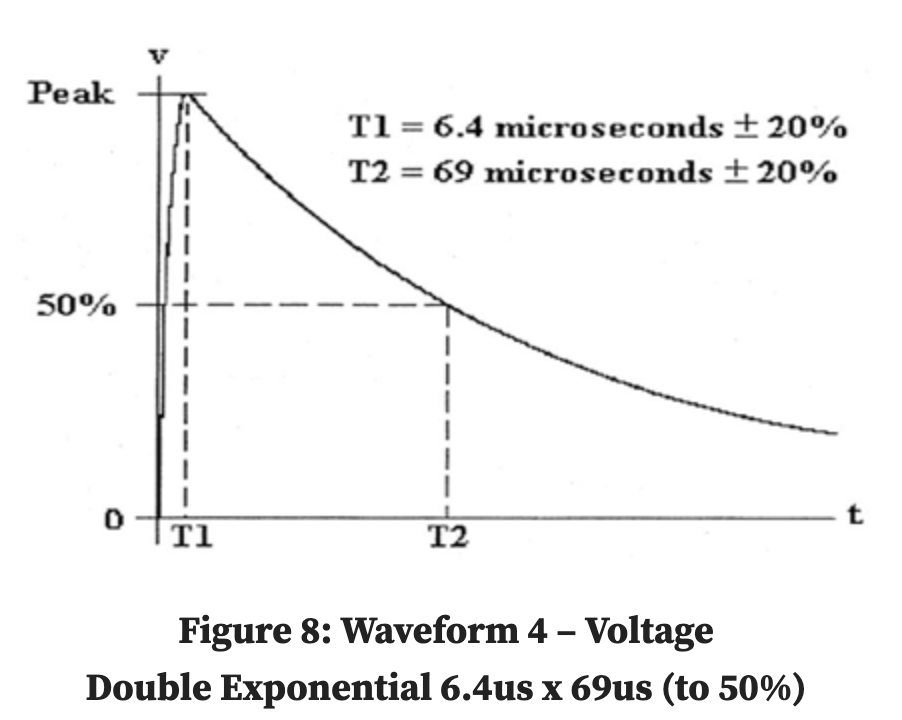
\includegraphics[width=1.0\linewidth]{do-160f_waveform_set_4.png}
    \caption{DO-160F Direct Pin Injection Lightning Test Waveform 4}
    \label{fig:do-160f_waveform_set_4_diagram}
\end{figure}

\section{Circuit Architecture}

\subsection{High-Level Overview}

For our team's circuit architecture, we did not follow an ideal AC-DC converter for our 115$V_{AC}$ - 28$V_{DC}$ bus, see Figure \ref{fig:ac_dc_converter_ideal_diagram}. Instead, a modified AC-DC converter was implemented that removed the transformer from the circuit; see Figure \ref{fig:ac_dc_converter_implemented_diagram}. Although an AC-DC converter may typically include a transformer to reduce common-mode noise when stepping down the $V_{AC}$, we decided to eliminate the component to increase the noise within the circuit's power path. As a team, we wanted to showcase the impact that proper filtering would have on load voltage and current. For industry, if weight and size were not constraints, then a transformer would likely be included.

\begin{figure}[htbp]
    \centering
    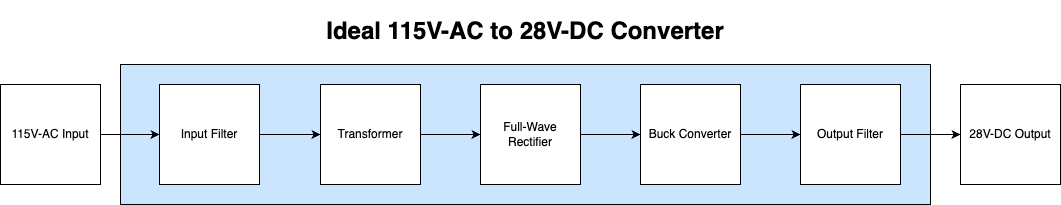
\includegraphics[width=1.0\linewidth]{ac_dc_converter_ideal.png}
    \caption{Ideal AC-DC Converter}
    \label{fig:ac_dc_converter_ideal_diagram}
\end{figure}

\begin{figure}[h]
    \centering
    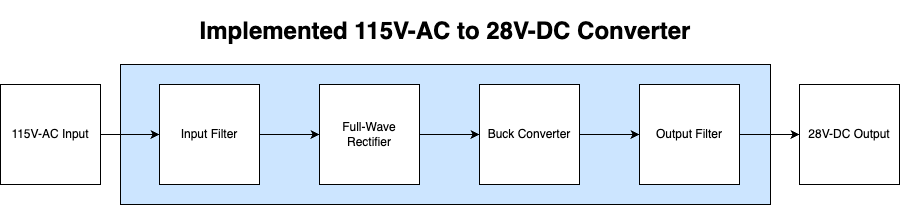
\includegraphics[width=1.0\linewidth]{ac_dc_converter_implemented.png}
    \caption{Implemented AC-DC Converter}
    \label{fig:ac_dc_converter_implemented_diagram}
\end{figure}

\subsection{Input Filter}

\subsection{Full-Wave Bridge Rectifier}
Directly after the AC input filters, the AC signal is fed into a full-wave bridge rectifier. The function of a full-wave rectifier is to convert the positive and negative half-cycles of an AC signal into a pulsating DC signal output, see Figure \ref{fig:full-wave_rectifier_output_waveform_diagram}. From there, a bulk capacitor is used on the output to "smooth" out the pulsating DC signal so that the output signal begins to resemble a stable DC output, see Figure \ref{fig:full-wave_bridge_rectifier_filter_waveform_diagram}. 

\begin{figure}[htp]
    \centering
    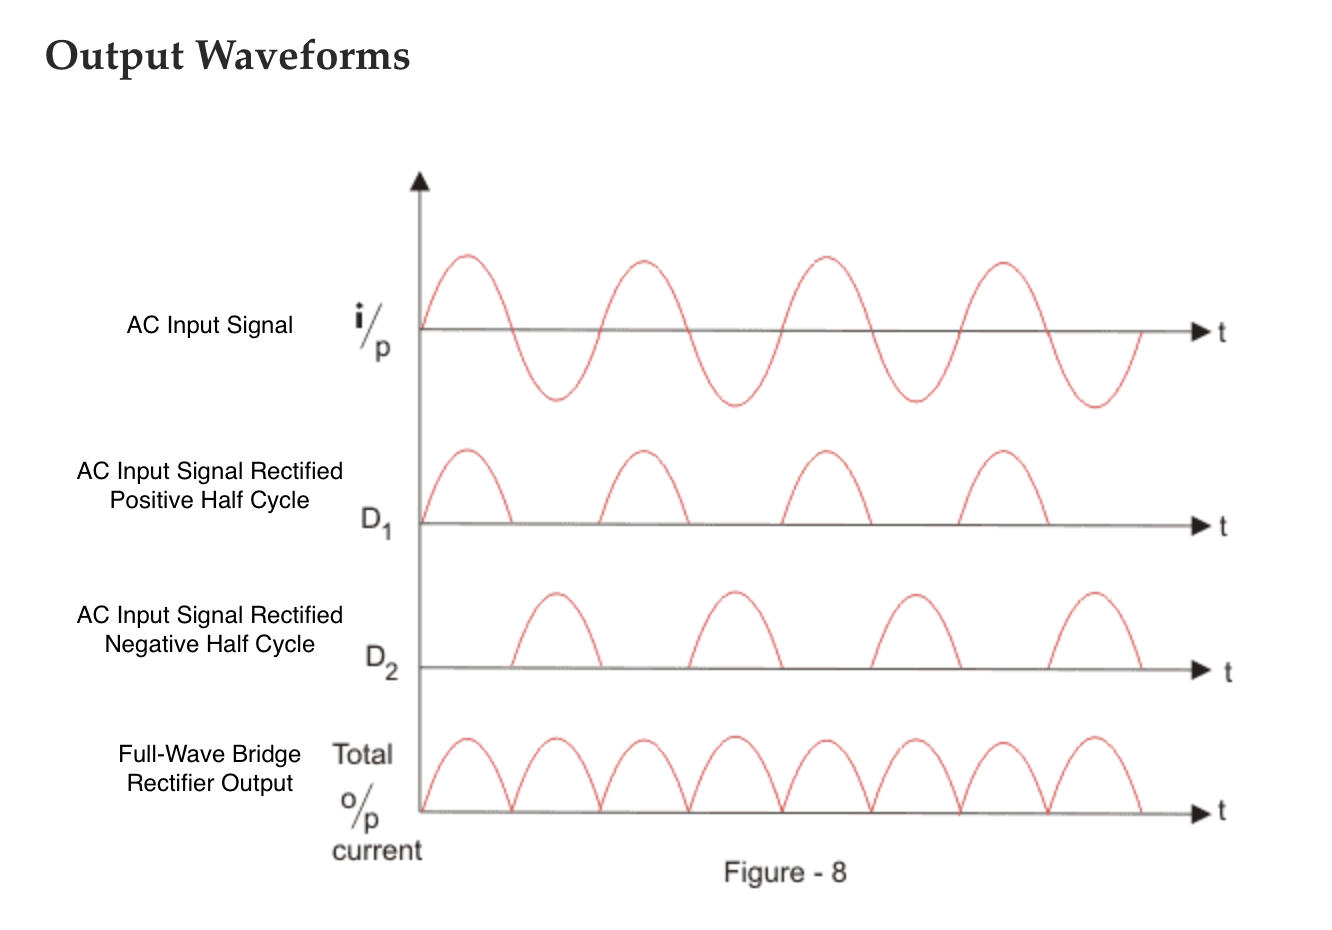
\includegraphics[width=1.0\linewidth]{full-wave_bridge_rectifier_output_waveform.png}
    \caption{Full-Wave Rectifier Output Waveforms}
    \label{fig:full-wave_rectifier_output_waveform_diagram}
\end{figure}

\begin{figure}[h]
    \centering
    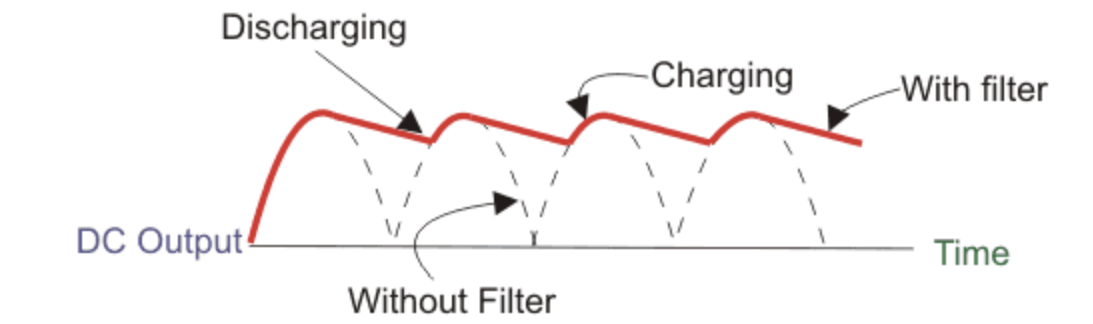
\includegraphics[width=1.0\linewidth]{full-wave_bridge_rectifier_filter_waveform.png}
    \caption{Full-Wave Rectifier Filter Waveform}
    \label{fig:full-wave_bridge_rectifier_filter_waveform_diagram}
\end{figure}


For our implementation, a full-wave bridge rectifier was implemented because it is more efficient than a half-wave rectifier. The LTSpice model is shown in Figure \ref{fig:full-wave_bridge_rectifier_circuit_diagram}. For a full-wave rectifier, both cycles of the AC signal are converted into the DC signal. For a half-wave rectifier, only a single half cycle of the AC signal is transferred, meanwhile the other half cycle is blocked. 

\begin{figure}[htp]
    \centering
    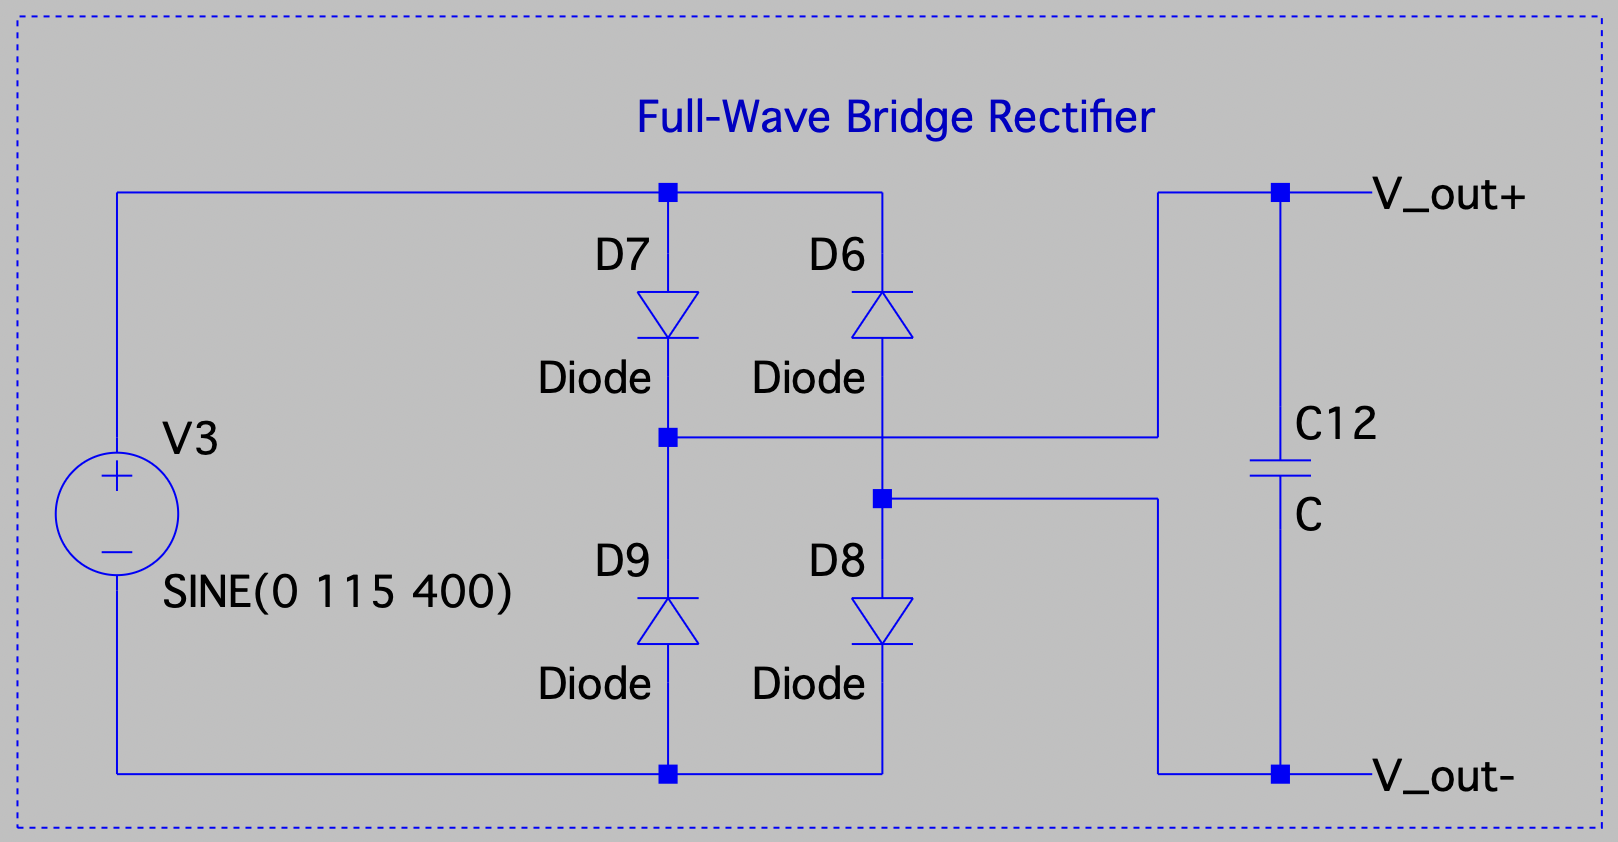
\includegraphics[width=1.0\linewidth]{full-wave_bridge_rectifier_circuit.png}
    \caption{Full-Wave Bridge Rectifier Circuit}
    \label{fig:full-wave_bridge_rectifier_circuit_diagram}
\end{figure}

\subsection{Buck Converter}
After the full-wave bridge rectifier is a Buck Converter. A buck converter is a DC-DC converter that steps down the DC input voltage using a voltage-controlled switch to generate a PWM output. After the PWM output, there is a bulk LC filter. The primary purpose of the bulk inductor and capacitor is to generate a stable stepped down DC output from the switching regulator's PWM input voltage. High-frequency noise introduced by the switching regulator will be handled by a separate block of output filtering components rather than by the bulk inductor and capacitor components. See Figure \ref{fig:buck_converter_circuit_diagram} for a diagram of a buck converter circuit.

\begin{figure}[htp]
    \centering
    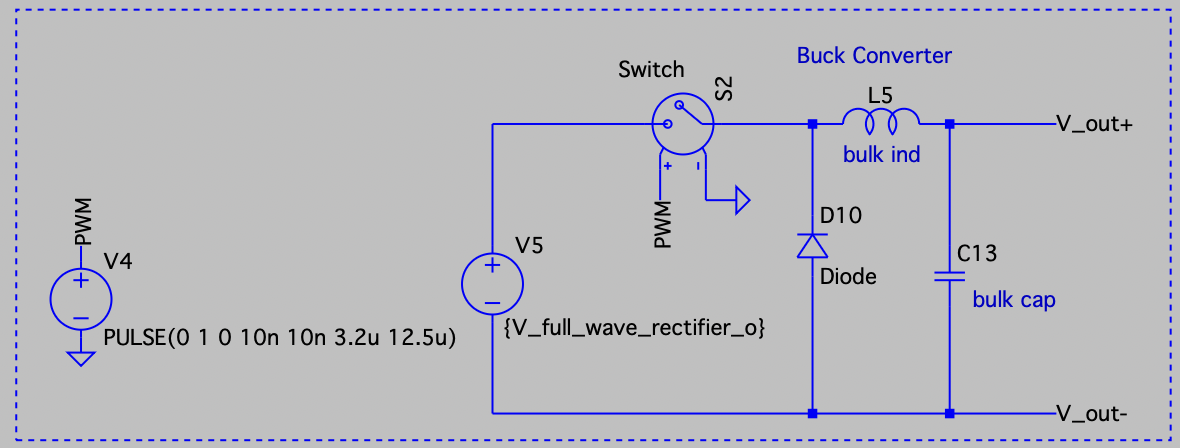
\includegraphics[width=1.0\linewidth]{buck_converter_circuit.png}
    \caption{Buck Converter Circuit}
    \label{fig:buck_converter_circuit_diagram}
\end{figure}

The bulk inductor resists changes in current, so when the switch is turned off, it attempts to keep the current constant. Meanwhile, the bulk capacitor resists changes in voltage, and thus attempts to keep the output voltage constant. The LC circuit includes a protection diode to prevent the switch from being damaged by a reverse voltage spike from the inductor's stored energy when the switch turns ON again. In contrast, when the switch is turned OFF, the forward bias of the protection diode allows the inductor to discharge its stored current. See Figure \ref{fig:buck_converter_waveform_diagram} for a diagram of the expected output waveforms of the buck converter.

\begin{figure}[htp]
    \centering
    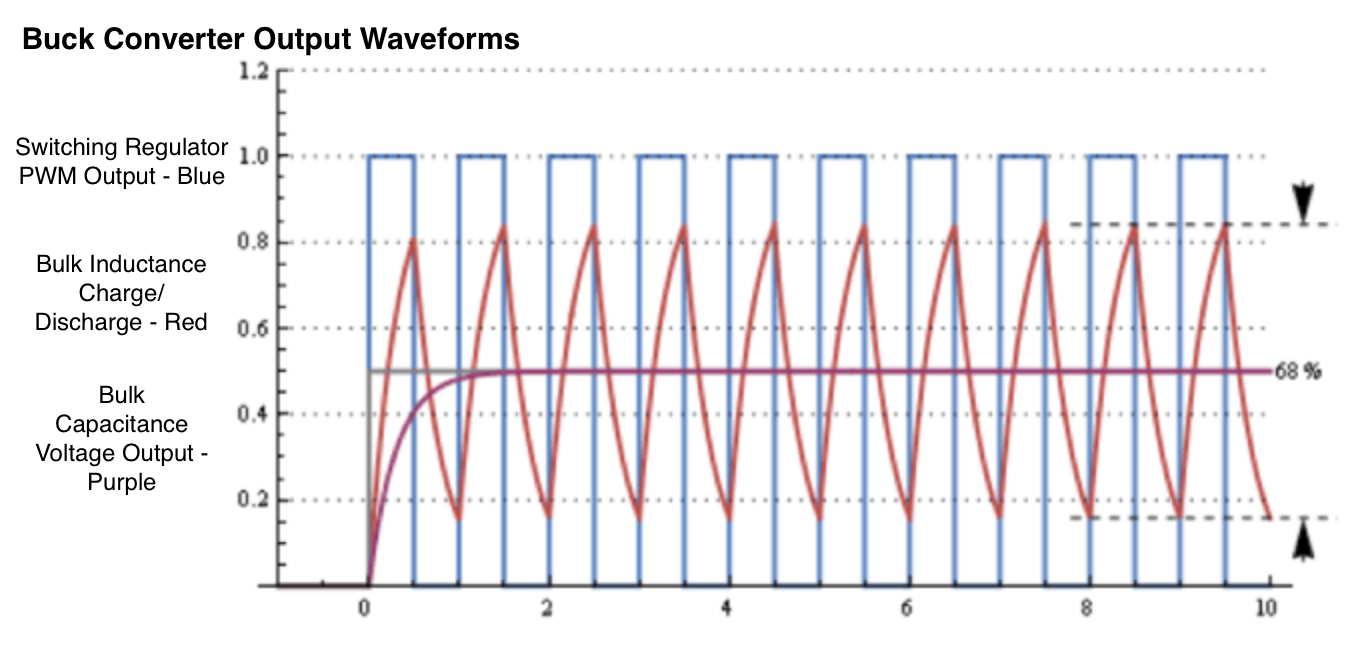
\includegraphics[width=1.0\linewidth]{buck_converter_waveform.png}
    \caption{Buck Converter Expected Output Waveform }
    \label{fig:buck_converter_waveform_diagram}
\end{figure}

Our group decided to move away from a linear regulator because the circuit is not as power-efficient as a switching regulator. The drawback of using a switching regulator is the voltage ripple introduced onto the DC output power rail due to the switching frequency. The switching noise and its harmonics will require output filtering to minimize the voltage ripple seen by the load and to guarantee that the conducted emissions of our circuit are below the DO-160G EMI conducted emissions threshold. 

The switching voltage regulator will not use a feedback loop for auto-adjustment of the switch's duty cycle. For a power rail, typically a feedback loop would be used to adjust the switch's duty cycle so that the power rail can maintain a 28$V_{DC}$ output across a range of loads. The scope of this course focuses on EMI compliance and circuit design, so the 28$V_{DC}$ output will be optimized to meet our 100$W$ power output in compliance with the DO-160G standard. If this were a power electronics course, then our team would have spent time to design a feedback loop to the switching regulator so that our 115$V_{AC}$ to 28$V_{DC}$ converter would be complaint across loads.

\subsection{Output Filter}

\section{Simulation Setup}
\subsection{Input Filter}
\subsection{Full-Wave Bridge Rectifier}
To model the full-wave bridge rectifier in LTSpice, t

\subsection{Buck Converter}
\subsubsection{Buck Converter Power Efficiency Estimation}
\subsubsection{LC Filter Calculation}
\subsection{Output Filter}


\section{Results}
\subsection{Input Filter}
\subsection{Full-Wave Bridge Rectifier}
\subsection{Buck Converter}
\subsection{Output Filter}
\subsection{Load}

\section{Discussion}
\subsection{Conducted Emissions at the Load}

\nocite{*}
\bibliographystyle{ieeetr}
\bibliography{final_project.bib}

\end{document}
